\chapter{Belle II}

Las herramientas que están en la vanguardia de los nuevos descubrimientos son las (súper) fábricas de B's de nueva generación como Belle II que es un experimento en el marco de la colaboración internacional Belle II donde participan  948 físicos e ingenieros de 26 países y 115 instituciones, entre las cuales se encuentra el Centro de Investigación y de Estudios Avanzados (CINVESTAV). Belle II es la mejora de Belle, en comparación, Belle II tomará entre 40 y 50 veces más datos que Belle, es decir mayor luminosidad. El sucesor de Belle es un espectrómetro magnético hermético rodeado de calorímetros, sistema de identificación de partículas y detectores de muones, optimizado para reconstruir colisiones electrón-positrón de 7 contra 4 GeV producidas por el colisionador SuperKEKB en Japón. SuperKEKB es el resultado de las mejoras realizadas en KEKB, un acelerador de leptones de 3016 m de circunferencia que logró alcanzar una cifra record de luminosidad instantánea de \(2.11\times10^{34}cm^{-2}s^{-1}\). Este tuvo un papel importantísimo a finales del siglo pasado, junto con el acelerador PEPII y su experimento BaBar en la confirmación del SM en el sector de sabor quark. En cuanto a SuperKEKB se espera lograr una luminosidad instantánea de alrededor de \(8\times10^{35}cm^{-2}s^{-1}\).

\section{Acelerador SuperKEKB}

SuperKEKB es un acelerador asimétrico de leptones, también se le puede denominar como una super fábrica de B's. Las fábricas de B's son denominadas así debido a que allí se producen colisiones electrón-positrón en la resonancia \(\Upsilon(4S)\), que es un estado quarkonio formado por un quark bottom y su antipartícula, pero en una resonancia que está justo en el umbral para la producción de mesones B a una energía del centro de masa (CM) de aproximadamente 10.58 \(GeV\). SuperKEKB acelera electrones en el anillo de alta energía (HER) de 7 GeV y positrones en el anillo de baja energía (LER) de 4 GeV, esto con el propósito de que dichas energías de haz asimétrico puedan proporcionar un boost al CM del sistema y de este modo permitir medidas de violación CP dependientes del tiempo. El boost es ligeramente inferior al de KEKB, lo cual es ventajoso para análisis con neutrinos y energía faltante en el estado final que requieren una buena hermeticidad del detector. La configuración del SuperKEKB se muestra en la figura  \ref{fig:superkekb}. Gracias al esquema de colisión de nano haz, que es una de las mejoras más importantes, se ha podido lograr las mejoras en la luminosidad ya que permite acelerar electrones y positrones enfocados en paquetes de 20 \(\mu m\) de ancho y 0.1 \(\mu m\) de alto (estos parámetros serán importantes en la reconstrucción de nuestro decaimiento), con este se puede compactar el haz 20 veces más que en KEKB. Para poder lograr esto, imanes cuadrupolares han sido instalados, además de imanes de corrección en el criostato e imanes de solenoide de compensación. También, se construyeron tubos cubiertos con TiN y la estructura de la autocámara para reducir la nube de fotoelectrones en el LER \cite{universe4100101}.
\begin{figure}[h]
    \centering
    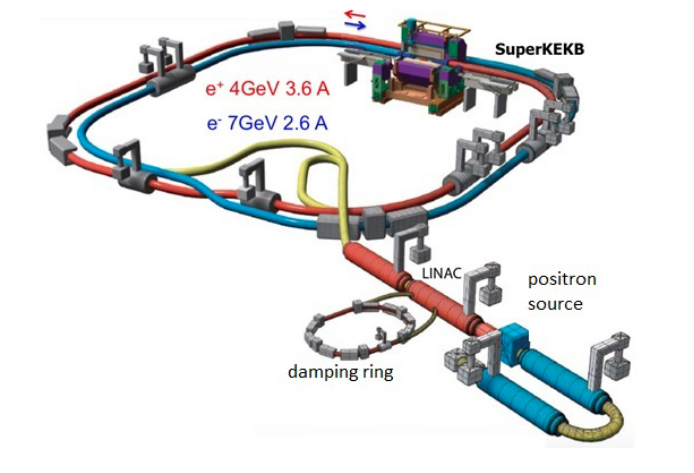
\includegraphics[scale=.5]{Images/superkekb.png}
    \caption{\small Vista esquemática del acelerador SuperKEKB.}
    \label{fig:superkekb}
\end{figure}

La luminosidad en SuperKEKB es determinada por tres parámetros que son: la corriente total de haz (\(I\)), el parámetro vertical de haz-haz (\(\xi_y\)) y la función beta del punto de interacción (\(\beta^{*}_{y}\)).   Dicha luminosidad se expresa en la siguiente fórmula asumiendo haces planos y componentes de haz verticales y horizontales iguales para dos haces en el punto de interacción (IP):
\begin{equation}
    L=\frac{\gamma_{\pm}}{2er_{e}}\left(\frac{I_{\pm}\xi_{y\pm}}{\beta^{*}_{y\pm}}\right)\left(\frac{R_{L}}{R_{\xi_{y}}}\right),
\end{equation}
donde \(\gamma_{\pm}\) es el factor de Lorentz, \(e\) la carga eléctrica fundamental, \(r_{e}\) el radio electrónico clásico, \(R_{L}\) y \(R_{\xi_{y}}\) factores de reducción para la luminosidad y el parámetro vertical de haz-haz respectivamente. El signo +(-) representa al positrón (electrón). En la tabla \ref{table:1} se sintetiza la elección de los 3 parámetros fundamentales, las energías de haz y la luminosidad para KEKB como para SuperKEKB.

\begin{table}[h!]
\centering
\begin{tabular}{|| c c c||} 
 \hline
  & KEKB & SuperKEKB \\ [0.5ex] 
 \hline\hline
 Energía (GeV) (LER/HER) & 3.5/8.0 & 4.0/7.0 \\ 
 \(\xi_{y}\) & 0.129/0.090 & 0.090/0.088  \\
 \(I\) (A) & 1.64/1.19 & 3.60/2.62   \\
 \(\beta^{*}_{y}\) (mm) & 5.9/5.9 & 0.27/0.41  \\
 Luminosidad (\(\times 10^{34}\) cm^{-2}s^{-1}) & 2.11 & 80  \\ [1ex] 
 \hline
\end{tabular}
\caption{Parámetros del antiguo KEKB y el actual SuperKEKB \cite{abe2010belle}.}
\label{table:1}
\end{table}

Actualmente SuperKEKB se encuentra en la segunda fase de toma de datos, logrando incrementar a un dataset de 100 \(fb^{-1}\), se espera también un pico de luminosidad instantánea para el 2025. La proyección de toma de datos y de luminosidad instantánea se puede ver en la siguiente figura.

\begin{figure}[h]
    \centering
    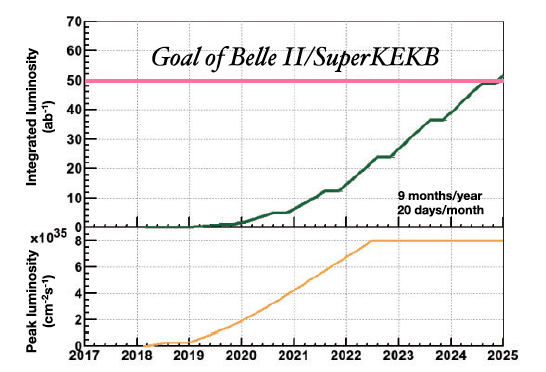
\includegraphics[scale=.5]{Images/Lumgoal.png}
    \caption{\small Proyección en la luminosidad que se espera alcanzar en SuperKEKB/Belle II.}
    \label{fig:superkekb}
\end{figure}

\section{Detector Belle II}

Para que las mejoras que se hicieron en el acelerador fuesen bien aprovechadas se requiere de un detector de gran nivel que esté equipado con los más sofisticados subdetectores que permitan con mayor eficiencia la detección de partículas cargadas y reconocimiento de trayectorias, así como un proceso de adquisición de datos (DAQ) eficaz. Ese detector es Belle II, una máquina de 1400 toneladas de 8 \(m\) de alto que se ubica en el punto de interacción (IP) de SuperKEKB. Su propósito es medir las trayectorias de las partículas producidas por los decaimientos de mesones (aunque no únicamente), identificarlas y reconstruir sus momentos y energías. Para mantener un excelente funcionamiento del espectrómetro se debe sortear un gran reto, mantener los efectos de los niveles de gran ruido mitigados, ya que al incrementar la luminosidad, el ruido de fondo crece de igual manera, este es un reto constante en Belle II, es por eso que los sistemas de trigger mejorados, los solenoides y  los sistemas de DAQ tienen una labor importantísima dentro del experimento. 

En múltiples aspectos, Belle II ofrece mejoras respecto a Belle, entre ellas están las siguientes:
\begin{itemize}
    \item los dispositivos de identificación de partículas en las regiones de barrel y de endcap amplían para los límites cinemáticos del experimento la región de separación de pión/kaón;
    \item la resolución de vértice mejoró por la excelente resolución espacial de las dos capas más internas del detector de píxeles;
    \item la eficiencia para la reconstrucción de los decaimientos de \(K_{s}\) a dos piones cargados que impactan en el detector de tiras de silicio, porque se mejora dicho detector al ocupar un mayor volumen;
    \item la nueva electrónica del calorímetro electromagnético (ECL) reduce considerablemente el ruido, lo cual es importante para estudios de energía perdida.
    
\end{itemize}
\newpage
Belle II es un detector construido en capas de subdetectores y componentes que dependiendo de su ubicación y los materiales de los cuales están hechos pueden detectar ciertos tipos de partículas y las trayectorias. El diseño escogido para Belle II se sintetiza en la imagen \ref{fig:belle2Config} y los cuales serán discutidos enseguida. Para una descripción detallada de todas las componentes de Belle II se recomienda revisar el Reporte de Diseño Técnico (TDR) \cite{abe2010belle}.

\begin{figure}[h]
    \centering
    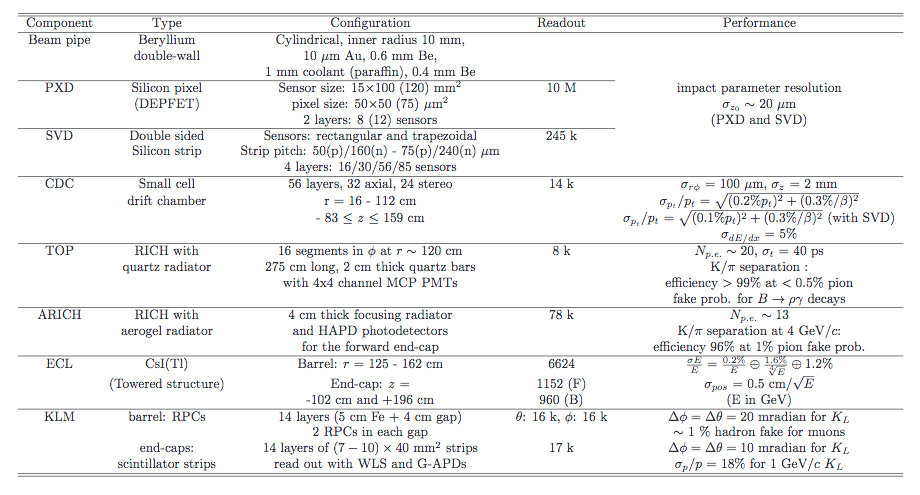
\includegraphics[scale=.5]{Images/BelleIIConfig.png}
    \caption{\small Componentes y detalles de diseño del espectrómetro Belle II \cite{abe2010belle}.}
    \label{fig:belle2Config}
\end{figure}
 En la imagen \ref{fig:belle2} podemos observar cómo se distribuyen los componentes y subdetectores de Belle II, así como su comparación con el tamaño de una persona promedio. El detector está conformado por un solenoide magnético superconductor,
el cual genera un campo magnético de 1.5 Tesla en el volumen del
detector, y siete elementos activos de detección: SVD, PXD, CDC, ECL, ARICH y
KLM.
 
 \begin{figure}[h]
    \centering
    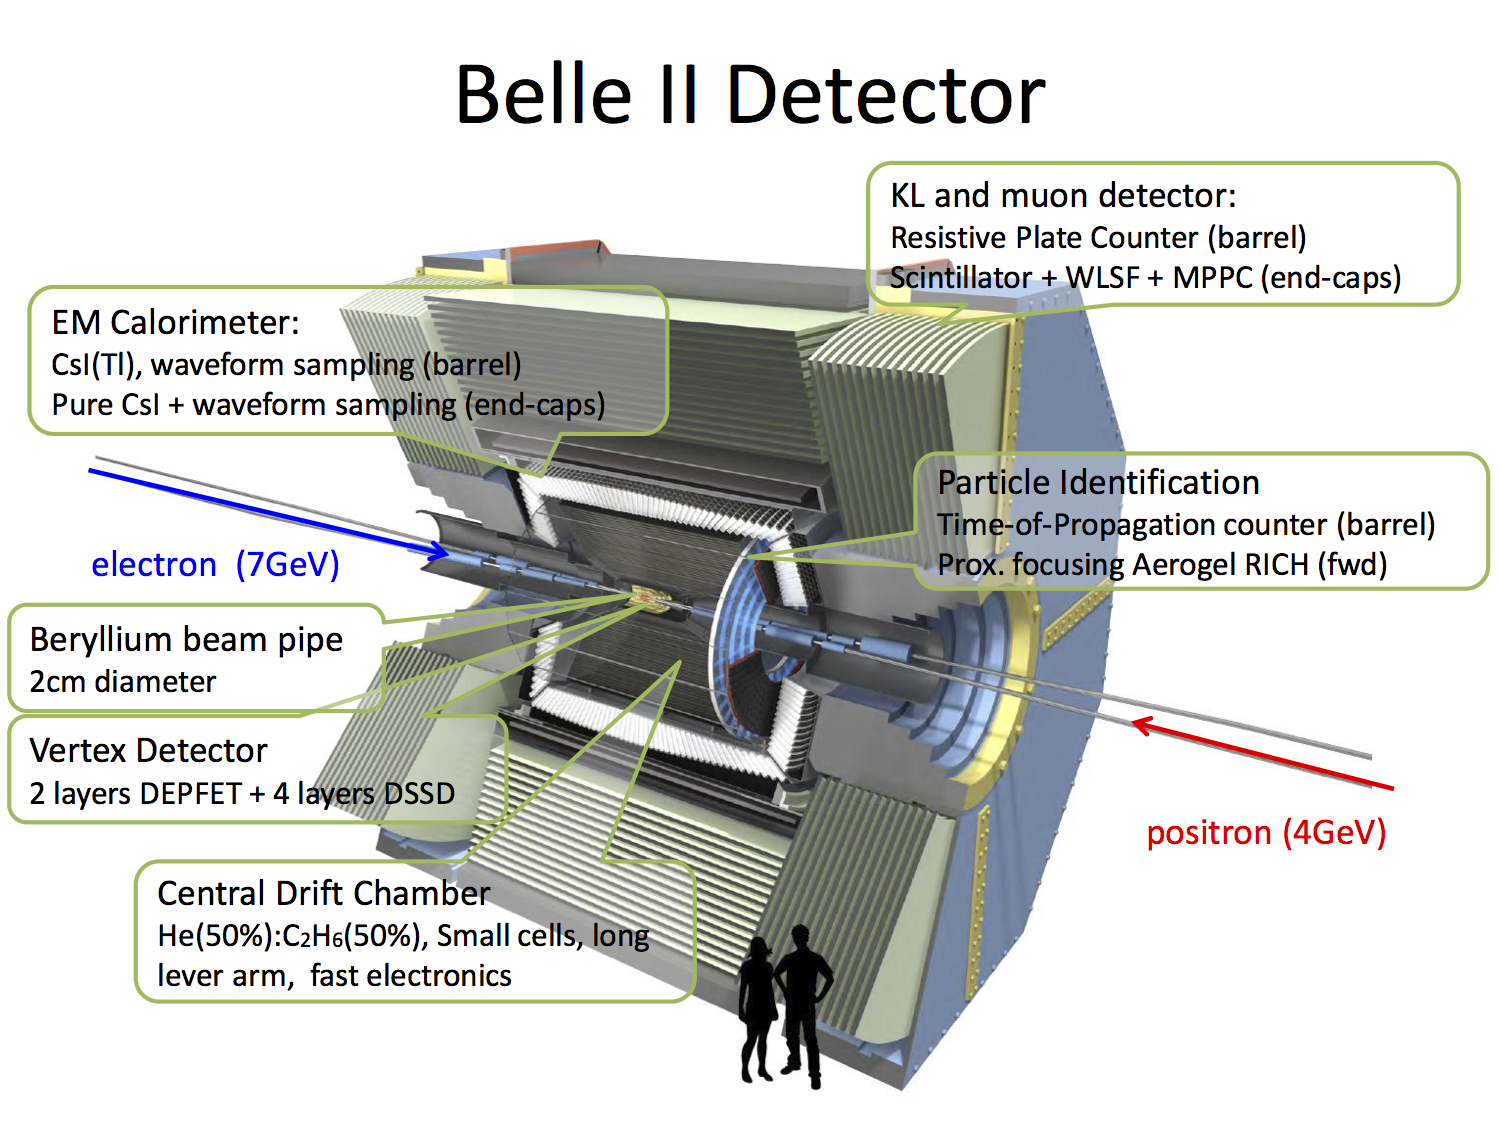
\includegraphics[scale=.5]{Images/belle2.png}
    \caption{\small Vista general del detector Belle II.}
    \label{fig:belle2}
\end{figure}

\newpage
\subsection{Detector de vértice VXD: PXD y SVD}

El VXD consiste en dos partes, la primera es el SVD (Silicon Vertex Detector) y la segunda es el PXD (Pixel Detector). Como se puede observar en la imagen \ref{fig:belle2Config} el VXD está compuesto de seis capas, las dos primeras que corresponden al PXD se ubican en \(r = 14\) mm y \(r = 22\) mm que usan sensores pixelados de tecnología DEPFET (DEPleted Field Effect Transistor) que permite sensores muy delgados (50 micras). Las cuatro capas restantes corresponden al SVD y se ubican en \(r = 39\) mm, \(r = 80 \) mm, \(r = 104\)  mm y \(r = 135\) mm, equipadas con detectores de tira de silicio de doble cara.

El PXD está optimizado para la reconstrucción de vértice de decaimientos de mesones B. El uso de transistores de efecto de campo los DEPFET para el PXD ofrece la ventaja de que no necesita una fuente de enfriamiento además del aire ya que debido a su pequeño espesor minimiza los efectos de dispersión, además permite tener una gran señal libre de ruido. Un dibujo en 3D del arreglo de los sensores del PXD se pueden ver en la figura \ref{fig:pxd}. Las medidas tan sensibles están determinadas también por la aceptancia de los requisitos angulares del tracker.
\begin{figure}[h]
    \centering
    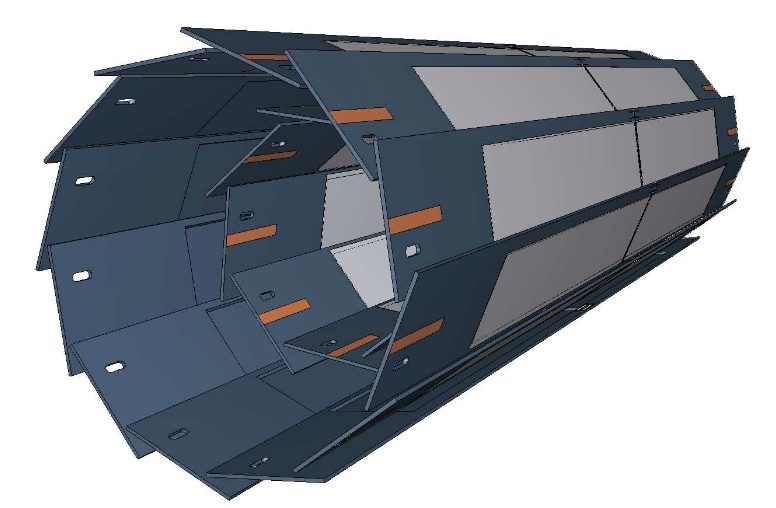
\includegraphics[scale=.4]{Images/pxd.png}
    \caption{\small Vista esquemática del arreglo geométrico de los sensores para el PXD.}
    \label{fig:pxd}
\end{figure}

El SVD por su parte consiste de cuatro capas de sensores ubicadas radialmente con un nivel de aceptancia angular de \(17^{\circ}<\theta<150^{\circ}\) y se encuentra ubicado entre el PXD y la cámara de deriva central (CDC), la geometría del SVD se puede observar en la imagen \ref{fig:svd}.

\begin{figure}[h]
    \centering
    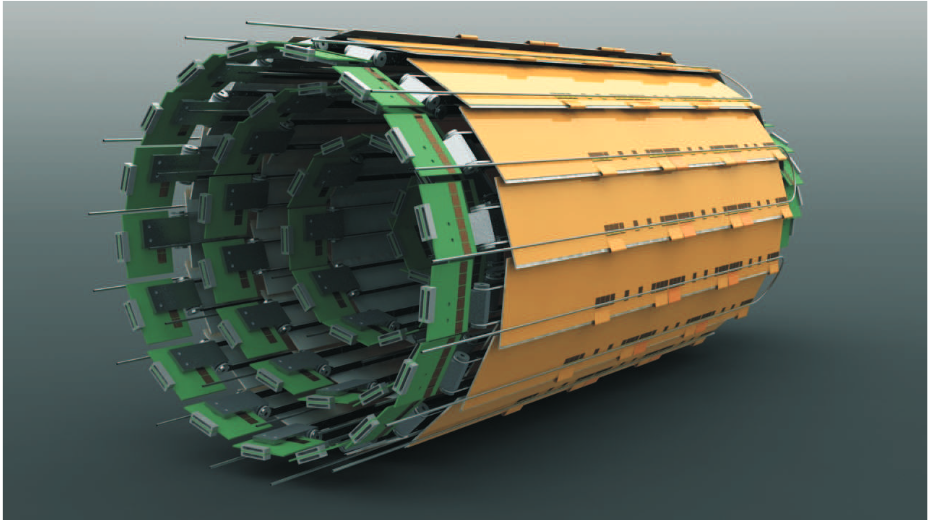
\includegraphics[scale=.4]{Images/svd.png}
    \caption{\small Vista esquemática del arreglo geométrico de los sensores para el SVD (4 capas)}
    \label{fig:svd}
\end{figure}

\subsection{Cámara de Deriva Central (CDC)}
Dentro del detector Belle II tenemos un instrumento fundamental, este es el dispositivo central de deteccción de partículas cargadas de gran volumen que se extiende a lo largo de un radio interno de 160 \(mm\) y externo de 1130 \(mm\), equipado con dispositivos de identificación de partículas (PID) más delgados comparados con los del antiguo Belle, dicho instrumento es el detector de cámara de deriva central que juega tres roles fundamentales dentro de Belle II. El primero de estos roles es la reconstrucción de los tracks cargados y la medida precisa de sus momentos, el segundo es proporcionar una información de identificación de partículas usando medidas de energías perdidas y tercero proporciona señales de activación eficientes y confiables para partículas cargadas. 

El CDC es un detector compuesto de 14336 celdas (ver figura \ref{fig:cdc}) con gas \(He-C_{2}H_{6}\) arregladas en 56 capas ubicadas axialmente (alineadas al campo magnético solonoidal) o estéreo (inclinadas respecto a las axiales). Por combinación de ambas configuraciones, axial y estéreo se logra reconstruir la trayectoria tridimensional completa de las partículas cargadas. En el eje z es asimétrico para que pueda estar de acuerdo a la asimetría en la energía de haz. El CDC de Belle II presenta mejoras con respecto al CDC Belle, brindando una mayor precisión en la determinación de la energía y el momento, así como de reconstrucción de trayectorias. También fue optimizado en la cantidad de material en la cámara para evitar la múltiple dispersión
\begin{figure}[h]
    \centering
    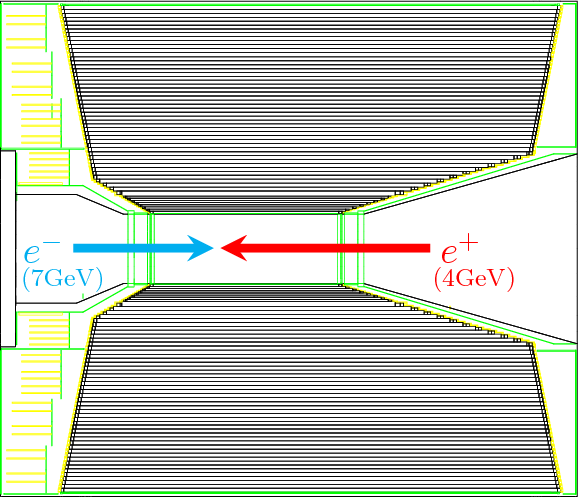
\includegraphics[scale=.5]{Images/CDC.png}
    \caption{\small Corte transversal en el CDC}
    \label{fig:cdc}
\end{figure}
\subsection{Sistema de identificación de partículas (PID): TOP y ARICH }
Para la identificación de partículas Belle II tiene en la región de barrel, un contador de tiempo de propagación (TOP) y el detector Cherenkov de imágenes de anillo de aerogel de enfoque de proximidad (ARICH) en la región de end-cap.

En la región de barrel se encuentra un tipo de detector Cherenkov, el TOP, constituido por barras de cuarzo (ver figura \ref{fig:top}) de 2.6 metros con dos filas de detectores de fotones alrededor de la pared externa del CDC arreglados en 16 módulos. Éste arreglo da información del tiempo de llegada y la posición de impacto de las partículas cargadas. En este contador, se mide el tiempo de propagación de los fotones Cherenkov que son internamente reflejados en los cuarzos. 
\begin{figure}%
    \centering
    \subfloat[\centering  ]{{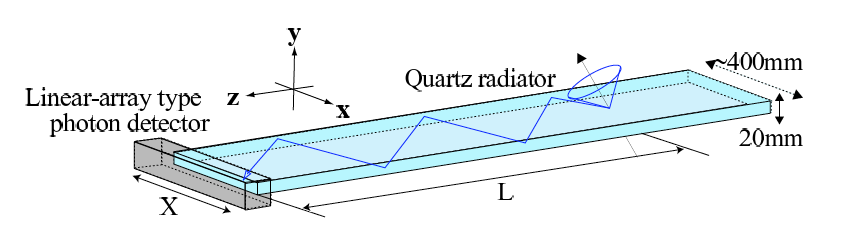
\includegraphics[width=7.5cm]{Images/TOP1.png} }}%
    \qquad
    \subfloat[\centering  ]{{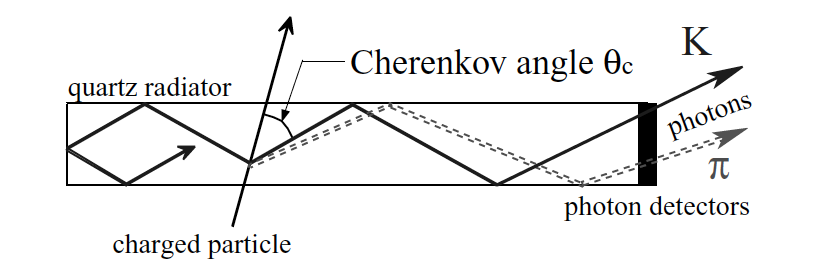
\includegraphics[width=7cm]{Images/TOP2.png} }}%
    \caption{(a) Diseño barra de cuarzo del detector TOP. (b) Vista esquemática de la reflexión interna en el contador TOP. \cite{abe2010belle}}%
    \label{fig:top}%
\end{figure}

La identificación de partículas cargadas sobre un rango cinemático completo es uno de los requisitos básicos para Belle II. En la tapa frontal, el detector ARICH ha sido diseñado para separar kaones de piones sobre la mayor parte de su espectro de momento (ver figura \ref{fig:arich}) y proporcionar una discriminación entre piones, muones y electrones por debajo de 0.4 \(GeV/c\) a 4 \(GeV/c\). Los elementos del ARICH son:

\begin{itemize}
    \item un radiador de aerogel donde los fotones Cherenkov son producidos por partículas cargadas;
    \item un volumen de expansión que permite que los fotones Cherenkov formen anillos sobre la superficie del detector de fotones;
    \item un arreglo de detectores de fotones sensibles a la posición, que es capaz de detectar fotones individuales en un gran campo magnético con gran frecuencia y con buena resolución en dos dimensiones;
    \item un sistema de lectura para el detector de fotones.
\end{itemize}

\begin{figure}%
    \centering
    \subfloat[\centering  ]{{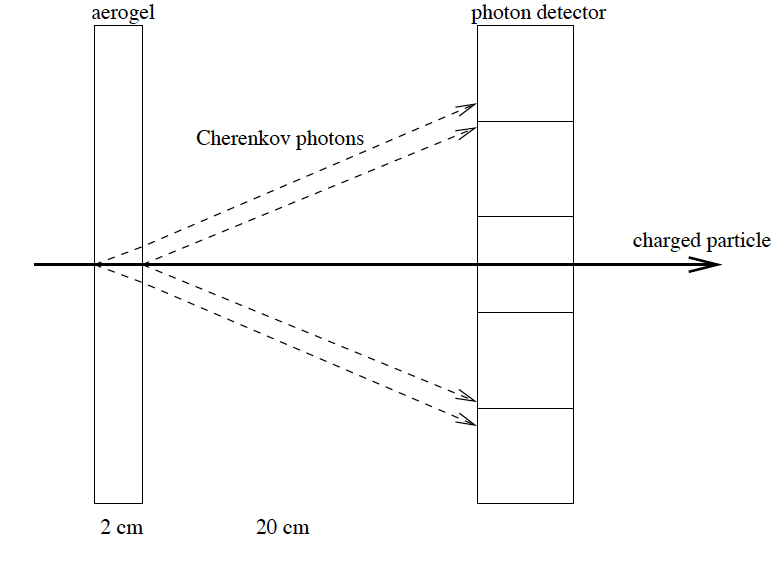
\includegraphics[width=7.3cm]{Images/ARICH.png} }}%
    \qquad
    \subfloat[\centering  ]{{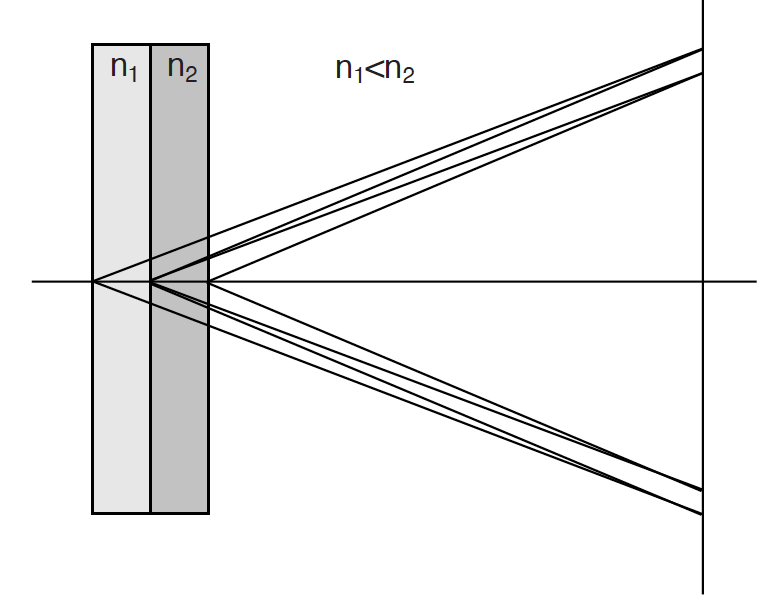
\includegraphics[width=6.5cm]{Images/ARICH2.png} }}%
    \caption{(a) Esquema de principio de funcionamiento del ARICH. (b) Esquema de las capas de aerogel con diferente índice de refracción del
detector ARICH. \cite{abe2010belle}}%
    \label{fig:arich}%
\end{figure}

Al elegir los índices de refracción de las capas de aerogel que se ubican consecutivamente de una manera óptima se puede lograr la superposición de los anillos Cherenkov correspondientes en el detector de fotones. De esta manera se logra el enfoque de fotones dentro del radiador, y se elimina o al menos reduce considerablemente la propagación debido a la incertidumbre del punto de emisión. Nótese que  el ajuste de índices de refracción sólo es posible con aerogel (debido a la versatilidad que este material ofrece), el cual debe ser producido con un índice de refracción en el rango de 1.01-1.2 \cite{abe2010belle}

\subsection{Calorímetro electromagnético (ECL)}

El ECL es un detector compuesto por un gran arreglo segmentado cristales de yoduro de cesio dopado con talio CsI(Tl) (8736 cristales en total), usado para detectar rayos gamma así como para identificar electrones, i.e, separar electrones de hadrones, en específico piones. Físicamente, el ECL es un detector en forma cilíndrica de unos 3 \(m\) de largo cuyo radio interno es de 1.25 \(m\) y tapas finales en \(z =\)1.96 \(m\) (hacia adelante) y \(z=\)-1.02 \(m\) (hacia atrás) desde el IP. Este detector cubre una región angular comprendida entre \(12.4^{\circ}<\theta<155.1^{\circ}\).

La parte central del ECL es reutilizado de Belle pero con algunas mejoras en la electrónica y el software de reconstrucción, ya que al incrementar la luminosidad, la cantidad de ruido aumenta, como ya se ha mencionado. Considerando que el tiempo de decaimiento relativamente largo del pulso de CsI(Tl) es fijo, al incrementar el ruido hay una superposición en los pulsos de eventos cercanos de ruido. Para contrarrestar esto se añadió a los fotodetectores discriminadores de forma de onda.

\subsection{Detector KLM}

El detector de \(K_{L}^{0}\) y muones es el más externo de Belle II, rodeando los detectores anteriormente descritos, el KLM consiste en placas de hierro de 4.7 \(cm\) de espesor ubicadas una sobre la otra, el conjunto de estas placas son llamadas cámara de placas resistivas (RPC's), el diseño del KLM se puede apreciar en la figura \ref{fig:klm}. Que sean de hierro las placas sirve para que regrese el flujo magnético al solenoide superconductor que se encuentra recubierto por el KLM. Como los \(K_{L}^0\) son partículas neutras pueden ser detectadas por medio de su interacción con la materia y por sus productos de decaimiento (ducha hadrónica), los muones pueden ser detectados ya que estos interactúan fácilmente con la materia. Con el propósito de minimizar la detección falsa de muones se instaló en las dos capas más internas del ECL centelladores.

\begin{figure}[h]
    \centering
    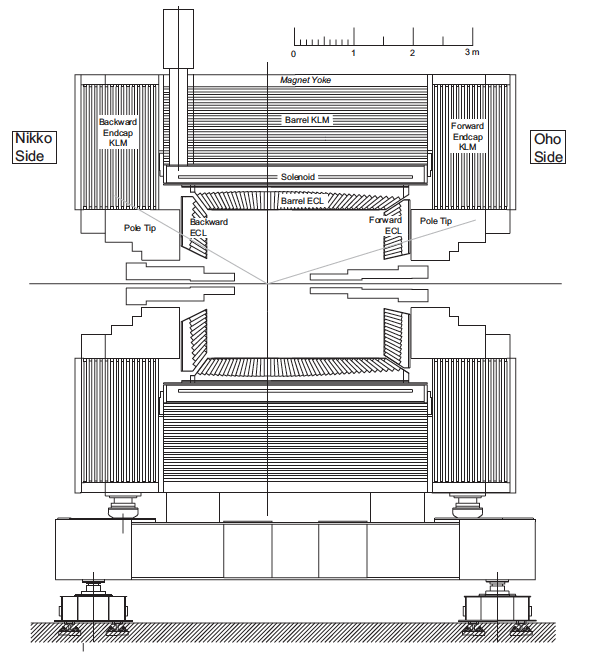
\includegraphics[scale=.5]{Images/KLM.png}
    \caption{\small Vista esquemática del detector KLM que se ubica en la parte externa de ECL.}
    \label{fig:klm}
\end{figure}

\subsection{Sistema de trigger}

Gracias a la alta luminosidad que se tiene en SuperKEKB es indispensable contar con un sistema de selección de datos, debido a la limitante y costo de almacenamiento que se requiere, el sistema de trigger en Belle II tiene un rol importante dentro del experimento. En Belle II se tiene un sistema de triggers dedicados que deben trabajar de la forma más eficiente posible, ya que de la gran cantidad de datos que se producen debido a un monto colosal de colisiones por segundo que ocurren, no todas se consideran de interés en la colaboración Belle II, los datos que son considerados de poco interés se catalogan como ruido. Así el sistema de trigger se consolida como la primera etapa de filtrado de datos. La selección de datos es llevada a cabo por medio de robustos sistemas electrónicos y de software (ver en la figura \ref{fig:trigger}) que procesan variables recolectadas en los detectores, de tal manera que al establecer valores particulares de estas y pedir que sólo los eventos que satisfagan ciertos requisitos de selección sean guardados, se consigue un mecanismo selector de datos. Además se debe tener en cuenta que los detectores tienen cierto tiempo de espera entre el registro de dos eventos, lo cual limitará la cantidad de datos que puede ser procesada. Por ejemplo, para la producción de taus se tiene una frecuencia de producción de 640 Hz y de detección de 30 Hz \cite{abe2010belle}.

El sistema de trigger de Belle II se constituye de dos niveles: el primero, un trigger de bajo nivel (L1) basado en hardware, y el segundo, un trigger de alto nivel basado en software (HLT). El trigger L1 tiene un tiempo de procesamiento de 5 \(\mu s\).
\begin{figure}[h]
    \centering
    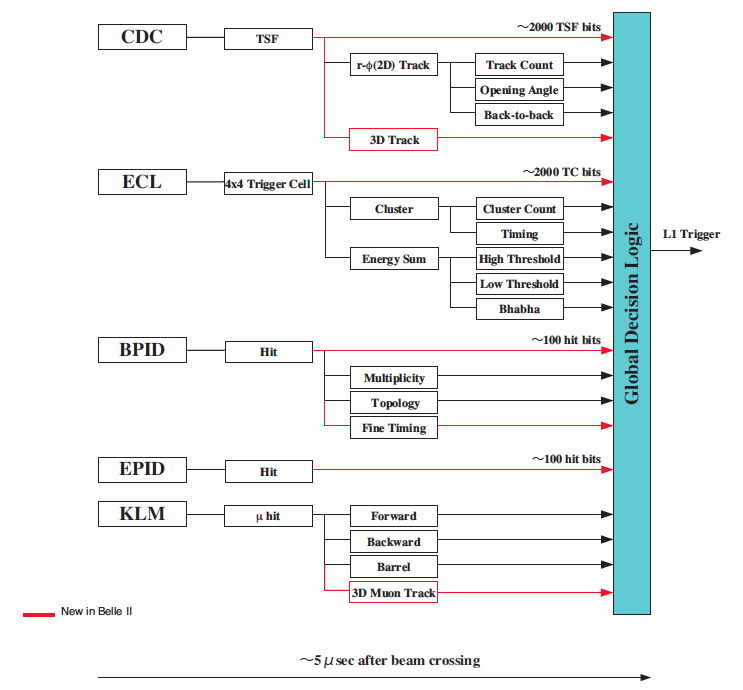
\includegraphics[scale=.6]{Images/trigger.png}
    \caption{\small Vista esquemática del sistema de trigger de Belle II \cite{abe2010belle}.}
    \label{fig:trigger}
\end{figure}
\subsection{Sistema DAQ}

El sistema de adquisición de datos (DAQ) en Belle II se encarga de leer los datos provenientes del trigger L1. El sistema se encarga de transferir los datos provenientes de la interfaz electrónica por medio de rigurosos pasos de procesamiento de datos que transforman estas señales análogas-electrónicas en señales digitales, para que posteriormente estos datos sean almacenados.

El proceso que se puede ver en la figura \ref{fig:daq} es el siguiente: después de la digitalización de los datos, estos se ubican cerca al detector y luego las señales digitalizadas pasan a una plataforma de lectura común llamada COPPER, esto por medio de un gran sistema de fibra óptica, este proceso de unificación del flujo de datos es denominado Belle2Link. Posteriormente, se efectúa una reducción de datos que pasan a los sistemas de PC's de lectura de salida (R/O PC), para luego entrar al nodo de construcción de eventos (Event Builder), donde se unen los datos provenientes de los distintos detectores para que formen bloques de información. Finalmente, los datos que son reducidos y con construcción de eventos pasan a ser procesados por el sistema de HLT por medio del software de selección de eventos. En este punto del proceso ya los datos pueden ser almacenados y en condiciones para ser analizados.
\begin{figure}[h]
    \centering
    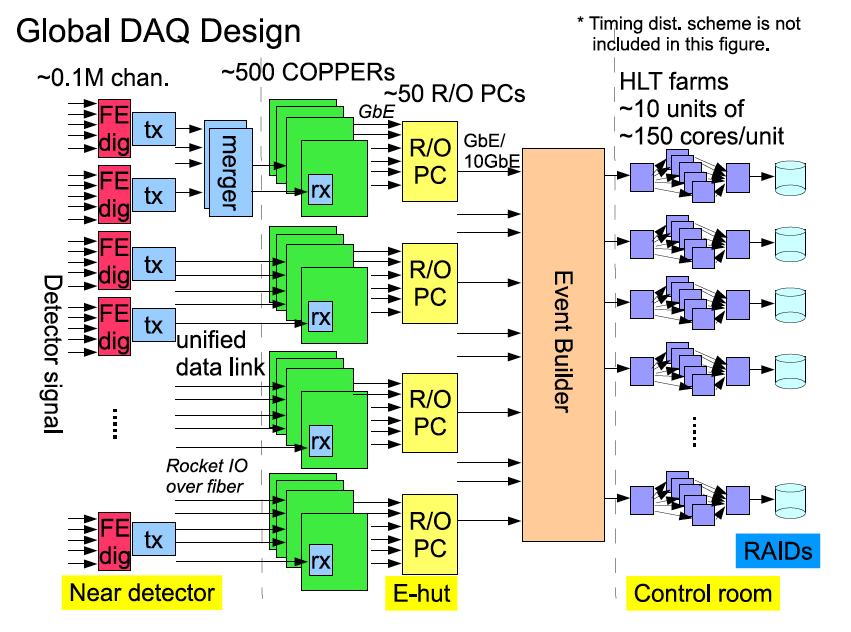
\includegraphics[scale=.5]{Images/DAQ.png}
    \caption{\small Diseño conceptual del sistema DAQ de Belle II \cite{abe2010belle}.}
    \label{fig:daq}
\end{figure} 
\subsection{Software de Belle II (Basf2)}

El software principal en Belle II es llamado Basf2, esta es una abreviación para ``Belle II Analysis Software Framework'' \cite{Kuhr2018}. Basf2 es un software para el manejo de grandes cantidades de datos construido en el lenguaje de programación C++, pero que su interfaz se basa en Python. En Belle II, Basf2 es usado en todas las etapas de procesamiento de datos, las cuales son: generación de datos simulados, desempaquetado de datos brutos reales, reconstrucción (como tracking, clustering, etc.) y reconstrucción de ``análisis'' de alto nivel (como aplicación de cortes, ajustes de vértices, etc.). Cabe resaltar que Basf2 no es utilizado para los pasos finales del análisis de datos (llenado de histogramas, ajustes de distribuciones 1D, entre otros); estos pasos finales suelen llamarse análisis ``offline'', donde generalmente se usa ROOT o Python.

Basf2 es un software que se construye a partir de módulos, que son piezas de código (usualmente) en C++ que utiliza una unidad específica de procesamiento de datos, los módulos están ordenados en una lista, a cual se le denomina camino (path). Por medio de los distintos paquetes y/o librerías se extraen los códigos para cada una de las etapas que se nombraron en el párrafo anterior, el espacio en donde se compendian con un orden lógico estas herramientas y se le dice al programa qué efectuar recibe el nombre de ``steering file'' o ``script''. El steering file o script es un código en Python que configura algunas de las tareas para el análisis o procesamiento de datos.

Además del procesamiento de datos, Basf2 cuenta con diferentes módulos para la generación de colisiones (EvtGen y KKMC)\cite{Lange:2001uf}\cite{Wa_s_2001}, por medio de PYTHIA \cite{Sj_strand_2015}. Para el caso en particular donde se trabaje con el leptón tau, los decaimientos son manejados por TAUOLA o su actualización, TAOLA-BBB. Es importante resaltar que estos generadores de eventos están basados en generación Monte Carlo \cite{Sjostrand:2006su}, es allí donde se producen eventos de decaimientos sin efectos de detector, ni cortes, ni ninguno de los aspectos relacionados con la selección de datos.

Para simular procesos que se asemejen a los ocurridos realmente en el detector se requiere de una herramienta que reproduzca los efectos de interacción de las partículas generadas con la materia, es en esta área donde el simulador GEANT4 \cite{GEANT4:2002zbu} es primordial, ya que este ayuda a reproducir las condiciones geométricas, interacciones con el campo magnético, pérdida de energía al atravesar los detectores, entre otras que enfrentan las partículas generadas en Belle II. GENT4 está implementado en el lenguaje C++ y ha sido importante en áreas de física de partículas, física nuclear, diseño de aceleradores y hasta en física médica.

\subsection{Análisis con ROOT}

Para el análisis offline de grandes cantidades de datos, luego que estos son adquiridos y filtrados por los distintos triggers se utiliza el software ROOT. El software está basado en el lenguaje C++ y permite la creación de histogramas, ajuste de distribuciones, análisis estadístico, creación de interfaz gráfica, etc. En esta tesis se usará ROOT para hacer el análisis y estimación de la masa para el leptón tau mediante el ajuste de los modelos propuestos \cite{Brun:1997pa}.